
创建库的工作方式与创建一个可执行文件的工作方式类似,但因为库目标通常是由其他目标使用的,要么在同一个项目中,要么由其他项目使用。因为库通常有一个内部和公开可见的API,所以在向项目添加文件时必须考虑到这一点。

简单的库项目是这样的:

\begin{lstlisting}[style=styleCMake]
cmake_minimum_required(VERSION 3.21)

project(
	ch3.hello_lib
	VERSION 1.0
	DESCRIPTION
	"A simple C++ project to demonstrate creating executables
	and libraries in CMake"
	LANGUAGES CXX)
	
add_library(hello)

target_sources(
	hello
	PRIVATE src/hello.cpp src/internal.cpp)
	
target_compile_features(hello PUBLIC cxx_std_17)

target_include_directories(
	hello
	PRIVATE src/hello
	PUBLIC include)
\end{lstlisting}

同样,该文件以设置\texttt{cmake\_minimum\_required}和项目信息开始,现在应该熟悉这些信息了。

接下来,使用\texttt{add\_library}创建库的目标——本例中,库的类型没有确定。可以传递\texttt{STATIC}或\texttt{SHARED}来显式确定库的类型,这里可以省略设置该类型,我们允许库的下游使用者可以选择如何构建和链接它。一般来说,静态库是最容易处理的。关于构建动态库的更多信息可以在“动态库的符号可见性”小节中找到。

如果省略了库的类型,则\texttt{BUILD\_SHARED\_LIBS}变量将决定库是默认构建为动态库还是静态库。这个变量不应该在项目的CMake文件中无条件地设置,应该总是由构建者传递。

使用\texttt{target\_sources}为库添加源文件。第一个参数是目标名称,后面跟\texttt{PRIVATE}、\texttt{PUBLIC}或\texttt{INTERFACE}关键字分隔相应源文件。实践中,源文件几乎总是使用\texttt{PRIVATE}添加,\texttt{PRIVATE}和\texttt{PUBLIC}关键字指定在何处使用源代码进行编译。指定\texttt{PRIVATE}意味着源文件将只在目标\texttt{hello}中使用。若使用\texttt{PUBLIC},那么源文件被添加到\texttt{hello}和链接到\texttt{hello}的目标上。正如前面提到的,这通常不是我们想要的结果。\texttt{INTERFACE}关键字意味着源文件不添加到\texttt{hello}目标,而是添加到任何链接到\texttt{hello}的目标。通常,为目标指定为\texttt{PRIVATE}的内容都可以视为构建需求。最后,库的包含目录使用\texttt{target\_include\_directories}设置。该指令指定的文件夹内的所有文件都可以使用\texttt{\#include <file.hpp>}(带尖括号),而非\texttt{\#include ""}来访问。

\texttt{PRIVATE}包含不会包含在目标属性中的路径,也就是\texttt{INTERFACE\_INCLUDE\_DIRECTORIES}。当目标依赖于该库时,CMake将读取该属性以确定哪些包含目录可见。

由于标准库的C++代码使用了与现代版本C++绑定的特性,如C++11/14/17/20或C++23(即将发布),我们必须设置\texttt{cxx\_std\_17}属性。由于用于编译库本身并与需要其接口,因此将其设置为\texttt{PUBLIC}。只有在头文件包含需要特定标准的代码时,才需要将其设置为\texttt{PUBLIC}或\texttt{INTERFACE}。若只有内部代码依赖于某个标准,则首选将其设置为\texttt{PRIVATE}。通常,尽量将公共C++标准设置为最低的可用标准,也可以只启用现代C++标准的某些特性。

完整的可用编译特性列表可参阅\url{https://cmake.org/cmake/help/latest/prop_gbl/CMAKE\_CXX\_KNOWN\_FEATURES.html}。

\subsubsubsection{3.4.1\hspace{0.2cm}命名库}

当使用\texttt{add\_library(<name>)}创建库时,库的名称在项目中必须全局唯一。默认情况下,库的实际文件名是根据平台上的约定构造的,例如\texttt{lib<name>}。在Linux上为<name>.lib,在Windows上为<名称>.dll。通过设置目标的\texttt{OUTPUT\_NAME}属性,可以更改文件的名称。这可以在下面的例子中看到,输出文件的名称已经从\texttt{ch3\_hello}改为\texttt{hello}:

\begin{lstlisting}[style=styleCMake]
add_library(ch3_hello)

set_target_properties(
	ch3_hello
	PROPERTIES OUTPUT_NAME hello
)
\end{lstlisting}

避免使用lib前缀或后缀的库的名称,因为CMake可能会在文件名后面或前面添加适当的字符串。当然,这取决于平台。

动态库的一种常用命名约定是在文件名中添加版本以指定构建版本和API版本,通过指定\texttt{VERSION}和\texttt{SOVERSION}属性,CMake将在构建和安装库时创建必要的文件名和符号链接:

\begin{lstlisting}[style=styleCMake]
set_target_properties(
	hello
	PROPERTIES VERSION ${PROJECT_VERSION} # Contains 1.2.3
	SOVERSION ${PROJECT_VERSION_MAJOR} # Contains only 1
)
\end{lstlisting}

Linux上,这个示例将导致libhello.so.1.0.0的文件名带有来自libhello的符号链接。所以,libhello.so.1指向实际的库文件。下面的截图展示了生成的文件和指向它的符号链接:

\begin{center}
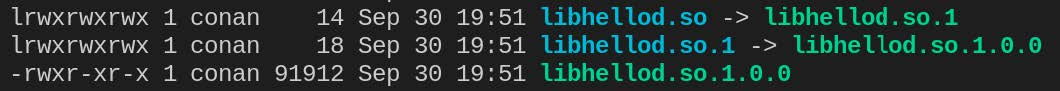
\includegraphics[width=1.\textwidth]{content/1/chapter3/images/1.jpg}\\
图3.1  使用SOVERSION属性构建库文件和生成的符号链接
\end{center}

项目中经常看到的另一种约定,是为各种构建配置的文件名添加不同的后缀。CMake通过设置\texttt{CMake \_<CONFIG>\_POSTFIX}全局变量或添加\texttt{<CONFIG>\_POSTFIX}属性来处理这个问题。若设置了此变量,后缀将自动添加到非可执行目标。与大多数全局变量一样,应该通过命令行传递给CMake,或者作为预置,而不是硬编码在CMakeLists.txt文件中。

调试库的后缀也可以显式地设置为单个目标,如下面的例子所示:

\begin{lstlisting}[style=styleCMake]
set_target_properties(
	hello
	PROPERTIES DEBUG_POSTFIX d)
\end{lstlisting}

这将导致库文件和符号链接命名为libhellod。由于在CMake中链接库是针对目标而不是文件名进行的,因此会自动选择正确的文件名,因此不必手动跟踪。然而,在链接动态库时要注意的是符号可见性。

\subsubsubsection{3.4.2\hspace{0.2cm}动态库中的符号可见性}

要链接到动态库,链接器必须知道哪些符号可以从库外部使用。这些符号可以是类、函数、类型等,使它们可见的过程称为导出。

指定符号可见性时,编译器有不同的方式和默认行为,这使得以独立于平台的方式指定符号可见性有点麻烦。从默认的编译器可见性开始;gcc和clang假设所有的符号都是可见的,而Visual Studio编译器默认情况下会隐藏所有的符号,除非显式导出。通过设置\texttt{CMAKE\_WINDOWS\_EXPORT\_ALL\_SYMBOLS},可以改变MSVC的默认行为,但这是一种暴力的解决方法,只有当一个库的所有符号都应该导出时才能使用。

虽然将所有的符号设置为公共可见是确保链接容易的一种简单方法,但它也有一些缺点:

\begin{itemize}
\item 
通过导出所有内容,就无法阻止依赖目标使用内部代码。

\item 
由于每个符号都可以被外部代码使用,链接器不能丢弃死代码,因此产生的库往往会膨胀。若库中包含模板,则尤其如此,因为模板往往会大幅增加符号的数量。

\item 
由于每个符号都是导出的,关于哪些应该被认为是隐藏的或内部的唯一线索必须来自文档。

\item 
暴露库的内部符号可能会暴露本应隐藏的东西。

\begin{tcolorbox}[colback=blue!5!white,colframe=blue!75!black,title=设置所有符号可见]
将动态库中的所有符号设置为可见时要小心,特别是在关心安全问题或二进制文件的大小很重要时。
\end{tcolorbox}
\end{itemize}

\hspace*{\fill} \\ %插入空行
\noindent
\textbf{更改默认可见性}

要更改符号的默认可见性,请将\texttt{<LANG>\_VISIBILITY\_PRESET}属性设置为\texttt{HIDDEN}。此属性可以全局设置,也可以针对单个库目标设置。\texttt{<LANG>}会替换为编写库的语言,例如:CXX替换为C++, C替换为C。若所有要导出的符号都是隐藏符号,必须在代码中被特别标记。最常见的方法是指定一个预处理器定义来确定一个符号是否可见:

\begin{lstlisting}[style=styleCXX]
class HELLO_EXPORT Hello {
	…
};
\end{lstlisting}

\texttt{HELLO\_EXPORT}定义将包含这样的信息:当编译库时,该符号是否导出,或者当对库进行链接时,它是否应该导入。GCC和Clang使用\texttt{\_\_attribute\_\_(…)}关键字来确定此行为,而在Windows上使用\texttt{\_declspec(…)}。编写以跨平台方式处理此问题的头文件并不是一项容易的任务,特别是若还必须考虑库可能构建为静态库和对象库。幸运的是,CMake提供了\texttt{generate\_export\_header}宏,由\texttt{GenerateExportHeader}模块导入。

下面的例子中,\texttt{hello}库的符号默认设置为隐藏。然后,通过使用\texttt{generate\_export\_header}宏再次单独启用。另外,本例将\texttt{VISIBILITY\_INLINES\_HIDDEN}属性设置为\texttt{TRUE},通过隐藏内联类成员函数来进一步减少导出符号表。设置内联的可见性不是严格必要的,但通常在设置了默认可见性后才会这样做:

\begin{lstlisting}[style=styleCMake]
add_library(hello SHARED)
set_property(TARGET hello PROPERTY CXX_VISIBILITY_PRESET
	"hidden")
set_property(TARGET hello PROPERTY VISIBILITY_INLINES_HIDDEN
	TRUE)
include(GenerateExportHeader)
generate_export_header(hello EXPORT_FILE_NAME export/hello/
	export_hello.hpp)

target_include_directories(hello PUBLIC "${CMAKE_CURRENT_
	BINARY_DIR} /export")
\end{lstlisting}

\texttt{generate\_export\_header}的调用在\texttt{CMAKE\_CURRENT\_BINARY\_DIR/export/hell}目录中创建了一个名为export\_hello.hpp的文件,该文件可以包含在库的文件中。将这些生成的文件放在构建目录的子文件夹中是一个好做法,这样只将目录的一部分添加到包含路径中。生成文件的include结构应该与库的其他部分的include结构匹配。因此,在这个例子中,通过\texttt{\#include <hello a\_public\_header.h>}来包含所有公共头文件,那么导出头文件也应该放在一个名为hello的文件夹中。生成的文件也必须添加到安装说明中,如第4章中所述。此外,要创建导出文件,必须将用于导出符号的必要编译器标志设置为目标。

因为生成的头文件必须包含在声明要导出的类、函数和类型的文件中,所以\texttt{CMAKE\_CURRENT\_BINARY\_DIR/export/}添加到\texttt{target\_include\_directories}中。注意,这必须是\texttt{PUBLIC},这样依赖库才可以找到该文件。

关于\texttt{generate\_export\_header}宏还有很多选项,但本节中看到的内容涵盖了大多数用例。关于设置符号可见性的其他信息,可以从官方CMake文档中检索到\url{https://cmake.org/cmake/help/latest/module/GenerateExportHeader.html}。

\subsubsubsection{3.4.3\hspace{0.2cm}接口或纯头文件库}

只有头文件的库有点特殊,因为它们不进行编译;相反,它们导出它们的头文件,以便直接包含在其他库中。大多数情况下,头文件库的工作方式与普通库类似,但是它们的头文件是使用\texttt{INTERFACE}关键字,而非\texttt{PUBLIC}关键字。

由于仅包含头文件的库不需要编译,因此不会向目标添加源文件。下面的代码创建了一个最小的头文件库:

\begin{lstlisting}[style=styleCMake]
project(
	ch3_hello_header_only
	VERSION 1.0
	DESCRIPTION "Chapter 3 header-only example"
	LANGUAGES CXX)

add_library(hello_header_only INTERFACE)
target_include_directories(hello_header_only INTERFACE
	include/)
target_compile_features( hello_header_only INTERFACE cxx_
	std_17)
\end{lstlisting}

值得注意的是,在CMake 3.19版本之前,\texttt{INTERFACE}库不能使用\texttt{target\_sources}。现在,头文件库可以不列出任何源文件。

\hspace*{\fill} \\ %插入空行
\noindent
\textbf{对象库——仅供内部使用}

有时,可能想要分离代码,以便部分代码可以重用,而不需要创建完整的库。当想在可执行测试和单元测试中使用某些代码时,通常的做法是不需要重新编译所有代码两次。为此,CMake提供了对象库,其中的源代码是编译的,但不进行归档或链接。通过\texttt{add\_library(MyLibrary object)}创建对象库。

自CMake 3.12起,这些对象可以像普通库一样使用,只需将它们添加到\texttt{target\_link\_libraries}函数中。在3.12版本之前,对象库需要添加生成器表达式,也就是\$<TARGET\_OBJECTS:MyLibrary>。这将在生成构建系统期间扩展为一个对象列表。这仍然可以完成,但不再推荐这样做,因为这很快就变得不可维护,特别是在一个项目中有多个对象库的情况下。

\begin{tcolorbox}[colback=blue!5!white,colframe=blue!75!black,title=何时使用对象库]
对象库可以在不公开模块的情况下加快代码的构建和模块化。
\end{tcolorbox}

使用对象库,可以覆盖所有不同类型的库。编写和维护库本身很有趣,但除非将它们集成到更大的项目中,否则它们什么也做不了。那么,让我们看看如何在可执行文件中,使用到目前定义的所有库。








